\documentclass[10pt,conference]{IEEEtran}
\IEEEoverridecommandlockouts
% The preceding line is only needed to identify funding in the first footnote. If that is unneeded, please comment it out.\usepackage{}


\usepackage{blindtext}

\usepackage{listings}

\usepackage{pifont}
\newcommand{\xmark}{\ding{55}}

\usepackage{xcolor}
\usepackage{tabularx}

% general imports
%\usepackage{amsmath,amssymb,amsfonts}

\usepackage{algorithmic}
\usepackage{graphicx}


% layout and formatting
\usepackage{microtype}

\usepackage{subcaption}

% configure hyperlinks 
\usepackage{hyperref}
\hypersetup{
	colorlinks,
	linkcolor={green!90!white},
	citecolor={blue},
	urlcolor={green!80!black}
}

% nice monospace font
%\usepackage{sourcecodepro}

%\usepackage{enumitem}


\usepackage{pdfcomment}

\usepackage{makecell}

\renewcommand\theadalign{bc}
\renewcommand\theadfont{\bfseries}
\renewcommand\theadgape{\Gape[0pt]}
\renewcommand\cellgape{\Gape[0pt]}

\usepackage{url}
\usepackage{float}

%nice font
%\usepackage{cochineal}


% configure subfigures
\usepackage{subcaption}

% configure tables
\usepackage{booktabs}
\usepackage{colortbl}

% table with footnotes
\usepackage{tablefootnote}



% fancy box for research questions, result summaries etc.
\usepackage[framemethod=TikZ]{mdframed}
\newcommand{\greybox}[1]{
	\begin{mdframed}[
		backgroundcolor=orange!0,
		linewidth=0.2pt,
		innerleftmargin=5pt,
		innertopmargin=5pt,
		roundcorner=2.5pt,
		]
		%\noindent
		#1
	\end{mdframed}
}


% remove indentioin for new paraghraphs
%\setlength{\parindent}{0cm}

% utility imports
\usepackage{comment}

\lstset{framesep=2pt}
\lstset{
	language=Java, 
	basicstyle=\footnotesize\ttfamily,
	linewidth=0.48\textwidth,
	numbers=left,
	columns=flexible,
	numbersep=5pt,      % Abstand der Nummern zum Text
	tabsize=2,
	%breaklines=true,
	%frame=bt,
	showspaces=false,
	showtabs=false,
	xleftmargin=10pt,
	breakatwhitespace=true,
	framexleftmargin=10pt,
	framexrightmargin=5pt,
	framexbottommargin=4pt,
	showstringspaces=false,
	literate=%
	{Ö}{{\"O}}1
	{Ä}{{\"A}}1
	{Ü}{{\"U}}1
	{ß}{{\ss}}2
	{ü}{{\"u}}1
	{ä}{{\"a}}1
	{ö}{{\"o}}1
}

\newcommand{\cova}{\makebox[0pt][l]{\color{red!15!white}\rule[-2pt]{0.92\textwidth}{8pt}}}
\newcommand{\covb}{\makebox[0pt][l]{\color{blue!15!white}\rule[-2pt]{0.92\textwidth}{8pt}}}
\newcommand{\covc}{\makebox[0pt][l]{\color{yellow!15!white}\rule[-2pt]{0.92\textwidth}{8pt}}}

% strikethrough
\usepackage[normalem]{ulem}



\usepackage{xargs} 
\usepackage[colorinlistoftodos,prependcaption,textsize=tiny]{todonotes}
\newcommandx{\unsure}[2][1=]{\todo[linecolor=red,backgroundcolor=red!25,bordercolor=red,#1]{#2}}
\newcommandx{\change}[2][1=]{\todo[linecolor=blue,backgroundcolor=blue!25,bordercolor=blue,#1]{#2}}
\newcommandx{\info}[2][1=]{\todo[linecolor=OliveGreen,backgroundcolor=OliveGreen!25,bordercolor=OliveGreen,#1]{#2}}
\newcommandx{\improvement}[2][1=]{\todo[linecolor=Plum,backgroundcolor=Plum!25,bordercolor=Plum,#1]{#2}}
\newcommandx{\thiswillnotshow}[2][1=]{\todo[disable,#1]{#2}}


\definecolor{duplicatecheck}{HTML}{ffd9d9}
\definecolor{autocommit}{HTML}{d9d9ff}
\definecolor{nicegreen}{HTML}{79c900}


\usepackage[most]{tcolorbox}

% color
% Custom commands for research questions
\newcommand{\RQ}[2]{
	\hypertarget{rq:#1}{
		\vspace{0.5em}
		\bgroup
		\def\arraystretch{1.3}%  1 is the default, change whatever you need
		\begin{tabularx}{\linewidth}{p{0.12\linewidth}|p{0.75\linewidth}}
			\rowcolor{
				orange!0}
			\textbf{RQ\,#1} & \textit{#2} \\
		\end{tabularx}
		\egroup
	}
}

%\colorbox{mentioned-color}{text}
\newcommand{\RQref}[1]{\hyperlink{rq:#1}{RQ\,#1}}

% Custom commands for subject systems
\usepackage{xspace}
\newcommand{\sosy}[1]{\textsc{\color{orange!50!black}#1}\xspace}
\newcommand{\jumper}{\sosy{jump3r}}
\newcommand{\htwo}{\sosy{h2}}
\newcommand{\hsqldb}{\sosy{hsqlsb}}
\newcommand{\kanzi}{\sosy{kanzi}}
\newcommand{\batik}{\sosy{batik}}
\newcommand{\dconvert}{\sosy{dconvert}}
\newcommand{\jadx}{\sosy{jadx}}


\def\BibTeX{{\rm B\kern-.05em{\sc i\kern-.025em b}\kern-.08em
		T\kern-.1667em\lower.7ex\hbox{E}\kern-.125emX}}


\begin{document}
	
\title{Analyzing the Impact of Workloads on Modeling the Performance of Configurable Software Systems}

\author{
	\centering
	\IEEEauthorblockN{
		Stefan Mühlbauer
	}
	\IEEEauthorblockA{
		\textit{Leipzig University}
	}
	\and
	\IEEEauthorblockN{
		Florian Sattler
	}
	\IEEEauthorblockA{
		\textit{Saarland University}\\
		\textit{Saarland Informatics Campus}
	}
	\and
	\IEEEauthorblockN{
		Christian Kaltenecker
	}
	\IEEEauthorblockA{
		\textit{Saarland University}\\
		\textit{Saarland Informatics Campus}
	}
	\and
	%\linebreakand
	\IEEEauthorblockN{
		Johannes Dorn
	}
	\IEEEauthorblockA{
		\textit{Leipzig University}
	}
	\and
	\linebreakand
	\IEEEauthorblockN{
		Sven Apel
	}
	\IEEEauthorblockA{
		\textit{Saarland University}\\
		\textit{Saarland Informatics Campus}
	}
	\and
	\IEEEauthorblockN{
		Norbert Siegmund
	}
	\IEEEauthorblockA{
		\textit{Leipzig University}\\
		\textit{ScaDS.AI Dresden/Leipzig}
	}
}

	
	
	\maketitle
	
	%\begin{IEEEkeywords}
	%	component, formatting, style, styling, insert
	%\end{IEEEkeywords}
	
	\maketitle
	\setcounter{tocdepth}{4}
	
	% abstract
	\begin{abstract}¸
	The artifacts described in this document refer to the study ``\textit{Analyzing the Impact of Workloads on Modeling the Performance of Configurable Software Systems}'' which explores how configuration options can influence software performance in conjunction with the workload.
	
	While the study presents a representative selection of the results, in this document, we provide as artifacts the experimental setup (software configurations and workload references) and observations (performance and coverage measurements). In addition, we provide an interactive dashboard that enables reproduction of analyses and visualizations. We make available all material via an archived software repository on \textit{zenodo.org}.
	\end{abstract}

	\section{Research Overview}
	Software systems can be customized through configuration options to enable desired functionality or improve non-functional aspects, such as performance or energy consumption. To estimate the performance of such systems, prediction models map a given configuration to an estimated performance value~\cite{pereira_2021_learning,kaltenecker_interplay_2020}. These models are based on a training set of configuration-specific performance measurements, which usually rely on only a single workload. However, previous work shows that the choice of workload, besides configuration, can significantly influence the performance of software systems in various ways~\cite{alves_sampling_2020,lesoil_2021}.  
	
	We conduct a systematic study that explores the quality and driving factors of the interaction between configuration options and workloads and their impact on software performance~\cite{muhlbauer_workload_2023}. In total, we analyze 25\,258 configurations and multiple workloads across nine real-world configurable software systems (\textsc{Java} and \textsc{C}/\textsc{C++}). We augment performance observations with code coverage information to explore driving causes for interactions between the workload and configuration options regarding their effect on software performance. 
	
	The study demonstrates that workloads can interact with configuration-specific performance, often in non-monotonous ways. This fact severely limits prediction models generalizability to arbitrary workloads. In addition, the observed sensitivity to the workload does not necessarily affect all configuration options equally, but is rather specific to individual configuration options. We identify workload-specific code coverage (i.e., code missed or covered only under specific workloads) as a partial cause for workload sensitivity.
	
	\section{Artifacts}
	To complement the representative selection of results~\cite{muhlbauer_workload_2023} and, to enable \textit{repoducibility} of our findings, we provide study artifacts (experimental data and an interactive dashboard for analyses and visualizations) via an archived software repository on \textit{zenodo.org}~\cite{muhlbauer_workload_2023_companion}:

	\subsection{Experiment Data}
	The experimental data provided comprises the study's experimental setup and measurements (performance and code coverage).
	
For the study, we selected nine configurable software systems. Each study subject exhibits configuration options along with constraints that we captured and provide as variability models in DIMACS (conjunctive normal form) notation. Configuration samples are drawn for each subject system using an ensemble of sampling strategies from our sampling library \textsc{SPLConqueror}\footnote{\textsc{SPLConqueror}: \url{https://www.se.cs.uni-saarland.de/projects/splconqueror/}} and provided as CSV files.
	Along with different configurations, we selected workloads for each subject system. Generally, we selected workloads that are inputs fed to and processed by the respective subject system (e.g., different files to compress or vector graphics to rasterize). We make available these resources via the companion repository.
	
	\subsubsection{Performance Measurements}
	For all data points (pairs of software configuration and workloads) we assess performance using either the utility \textsc{GNU time} (execution time) or \textsc{OLTPBench}~\cite{difallah_oltp_2013} (throughput). All measurements were orchestrated using the workload manager \textsc{Slurm}\footnote{\textsc{Slurm}: \url{https://slurm.schedmd.com/}} and conducted on compute clusters with a headless \textsc{Debian} installation and identical hardware setup across each cluster, respectively. We provide all performance observations as CSV files via the companion repository.
	
	\subsubsection{Code Coverage Measurements}
	In addition, we conducted for all data points a separate run to collect code coverage information. For \textsc{Java} subject systems, we employed the on-the-fly profiler \textsc{JaCoCo}\footnote{\textsc{JaCoCo}: \url{https://www.jacoco.org/jacoco/trunk/doc/}}, whereas for \textsc{C/C++} systems, we collected coverage information from executing binary build with instrumentation code using LLVM\footnote{\textsc{LLVM}: \url{https://clang.llvm.org/docs/SourceBasedCodeCoverage.html}}. We provide all line coverage information (per data point) via the companion repository.
		
	\subsection{Interactive Dashboard}
	In the study, we analyzed the data with regard to the quality of interactions between the workload and configurations ($\text{RQ}_\text{1}$), the workload sensitivity of individual configuration options ($\text{RQ}_\text{2}$), and the potential relationship between workload sensitivity and workload-specific code coverage ($\text{RQ}_\text{3}$). To explore the vast data set more easily, we implemented the corresponding analyses via an interactive dashboard. All result visualizations presented in the study~\cite{muhlbauer_workload_2023} can be generated from this dashboard as well as those omitted due to space limitations. This way, the dashboard not only complements the presentation of results in the study, but provides a means to reproduce analyses and reenact findings from our study.
	
	\begin{figure}
		\centering
		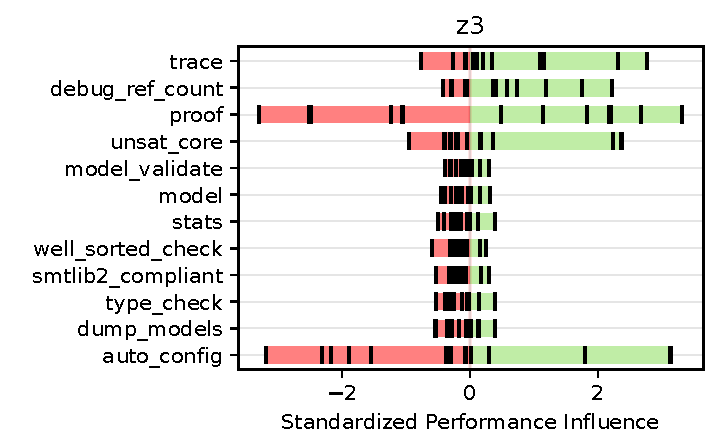
\includegraphics[width=\linewidth]{images/z3.pdf}
		\caption{Hier könnte Ihre caption stehen}
	\end{figure}
	
	The dashboard application is implemented using the \textsc{Python} framework \texttt{streamlit} and is provided as a containerized application (Docker) via the companion repository.
	
	
	%\clearpage
	%\color{black}
	\bibliographystyle{IEEEtran}
	\bibliography{literature}
\end{document}
